%%%%%%%%%%%%%%%%%%%%%%%%%%%%%%%%%%%%%%%%%
% University Assignment Title Page 
% LaTeX Template
% Version 1.0 (27/12/12)
%
% This template has been downloaded from:
% http://www.LaTeXTemplates.com
%
% Original author:
% WikiBooks (http://en.wikibooks.org/wiki/LaTeX/Title_Creation)
%
% License:
% CC BY-NC-SA 3.0 (http://creativecommons.org/licenses/by-nc-sa/3.0/)
% 
% Instructions for using this template:
% This title page is capable of being compiled as is. This is not useful for 
% including it in another document. To do this, you have two options: 
%
% 1) Copy/paste everything between \begin{document} and \end{document} 
% starting at \begin{titlepage} and paste this into another LaTeX file where you 
% want your title page.
% OR
% 2) Remove everything outside the \begin{titlepage} and \end{titlepage} and 
% move this file to the same directory as the LaTeX file you wish to add it to. 
% Then add %%%%%%%%%%%%%%%%%%%%%%%%%%%%%%%%%%%%%%%%%
% University Assignment Title Page 
% LaTeX Template
% Version 1.0 (27/12/12)
%
% This template has been downloaded from:
% http://www.LaTeXTemplates.com
%
% Original author:
% WikiBooks (http://en.wikibooks.org/wiki/LaTeX/Title_Creation)
%
% License:
% CC BY-NC-SA 3.0 (http://creativecommons.org/licenses/by-nc-sa/3.0/)
% 
% Instructions for using this template:
% This title page is capable of being compiled as is. This is not useful for 
% including it in another document. To do this, you have two options: 
%
% 1) Copy/paste everything between \begin{document} and \end{document} 
% starting at \begin{titlepage} and paste this into another LaTeX file where you 
% want your title page.
% OR
% 2) Remove everything outside the \begin{titlepage} and \end{titlepage} and 
% move this file to the same directory as the LaTeX file you wish to add it to. 
% Then add %%%%%%%%%%%%%%%%%%%%%%%%%%%%%%%%%%%%%%%%%
% University Assignment Title Page 
% LaTeX Template
% Version 1.0 (27/12/12)
%
% This template has been downloaded from:
% http://www.LaTeXTemplates.com
%
% Original author:
% WikiBooks (http://en.wikibooks.org/wiki/LaTeX/Title_Creation)
%
% License:
% CC BY-NC-SA 3.0 (http://creativecommons.org/licenses/by-nc-sa/3.0/)
% 
% Instructions for using this template:
% This title page is capable of being compiled as is. This is not useful for 
% including it in another document. To do this, you have two options: 
%
% 1) Copy/paste everything between \begin{document} and \end{document} 
% starting at \begin{titlepage} and paste this into another LaTeX file where you 
% want your title page.
% OR
% 2) Remove everything outside the \begin{titlepage} and \end{titlepage} and 
% move this file to the same directory as the LaTeX file you wish to add it to. 
% Then add %%%%%%%%%%%%%%%%%%%%%%%%%%%%%%%%%%%%%%%%%
% University Assignment Title Page 
% LaTeX Template
% Version 1.0 (27/12/12)
%
% This template has been downloaded from:
% http://www.LaTeXTemplates.com
%
% Original author:
% WikiBooks (http://en.wikibooks.org/wiki/LaTeX/Title_Creation)
%
% License:
% CC BY-NC-SA 3.0 (http://creativecommons.org/licenses/by-nc-sa/3.0/)
% 
% Instructions for using this template:
% This title page is capable of being compiled as is. This is not useful for 
% including it in another document. To do this, you have two options: 
%
% 1) Copy/paste everything between \begin{document} and \end{document} 
% starting at \begin{titlepage} and paste this into another LaTeX file where you 
% want your title page.
% OR
% 2) Remove everything outside the \begin{titlepage} and \end{titlepage} and 
% move this file to the same directory as the LaTeX file you wish to add it to. 
% Then add \input{./title_page_1.tex} to your LaTeX file where you want your
% title page.
%
%%%%%%%%%%%%%%%%%%%%%%%%%%%%%%%%%%%%%%%%%

%----------------------------------------------------------------------------------------
%	PACKAGES AND OTHER DOCUMENT CONFIGURATIONS
%----------------------------------------------------------------------------------------

\documentclass[12pt, showidx]{article}

\usepackage[utf8]{inputenc}
\usepackage[T1]{fontenc}
\usepackage{lmodern}
\usepackage{parselines}
\usepackage[portuguese]{babel}
\usepackage{graphicx}
\usepackage{imakeidx}
\usepackage[document]{ragged2e}

\graphicspath{ {images/} }

\makeindex[title = Palavras Chave]

\begin{document}

\begin{titlepage}

\newcommand{\HRule}{\rule{\linewidth}{1mm}} % Defines a new command for the horizontal lines, change thickness here

\center % Center everything on the page
 
%----------------------------------------------------------------------------------------
%	HEADING SECTIONS
%----------------------------------------------------------------------------------------


\includegraphics{feup.jpg}

\textsc{\large Inteligência Artificial}\\[0.5cm] % Major heading such as course name
\textsc{\large 3º ano do Mestrado Integrado em Engenharia Informática e Computação}\\[0.5cm] % Minor heading such as course title

%----------------------------------------------------------------------------------------
%	TITLE SECTION
%----------------------------------------------------------------------------------------

\HRule \\[0.4cm]
{ \huge \bfseries Otimização da gestão de projetos}\\[0.2cm] % Title of your document
\HRule \\[1cm]
 
%----------------------------------------------------------------------------------------
%	AUTHOR SECTION
%----------------------------------------------------------------------------------------


% If you don't want a supervisor, uncomment the two lines below and remove the section above
\Large \emph{Authors:}\\
Duarte \textsc{Pinto}\\[0cm] - up201304777 
- up201304777@fe.up.pt\\[0cm]
Filipa \textsc{Ramos}\\[0cm] - up201305378
- up201305378@fe.up.pt\\[0cm] 
Gustavo \textsc{Silva}\\[0cm] - up201304143
- up201304143@fe.up.pt\\[1cm] % Your name

%----------------------------------------------------------------------------------------
%	DATE SECTION
%----------------------------------------------------------------------------------------

{\large \today}\\[0cm] % Date, change the \today to a set date if you want to be precise

%----------------------------------------------------------------------------------------
%	TABLE OF CONTENTS & LISTS OF FIGURES AND TABLES
%----------------------------------------------------------------------------------------

\tableofcontents

%----------------------------------------------------------------------------------------
%	INTRODUÇÃO
%----------------------------------------------------------------------------------------

\section{Introdução} 

\justify\normalsize
No âmbito da unidade curricular de Inteligência Artificial pretende-se desenvolver um programa que, com base em algoritmos genéticos e arrefecimento simulado, faça a gestão de um projeto balançando os elementos participantes e as tarefas a realizar do mesmo. O sistema é composto por um conjunto de tarefas que pertencem ao projeto em análise. Cada tarefa tem uma competência indispensável ao seu cumprimento e uma duração. Cada elemento tem um conjunto de competências sendo que o mesmo tem um nível de capacidade para cumprir cada uma. A gestão a ser realizada tem em vista minimizar o tempo ocupado para satisfazer todas as tarefas do projeto usando a melhor combinação de elementos para cada tarefa. Será feita uma análise comparativa entre o desempenho das solução encontradas com algoritmos genéticos e arrefecimento simulado. 

Os objetivos principais do projeto passam pela exploração da implementação prática dos algoritmos genéticos e do algoritmo de arrefecimento simulado. Através dos dados obtidos, visa-se também realizar uma comparação da solução encontrada com ambos os algoritmos. Este processo irá fomentar o conhecimento adquirido, evidenciando as vantagens principais de cada algoritmo e as suas dicotomias principais.  

Espera-se que surjam dificuldades na implementação prática dos algoritmos estudados teoricamente, principalmente na construção dos cromossomas pois existem dúvidas em relação à sua influência na eficiência da solução encontrada. Para além disto, a melhor adaptação da função de avaliação ao problema por forma a obter os melhores resultados revela-se um processo tumultuoso. Os membros decidiram optar por otimizar o tempo utilizado a concluir todas as tarefas do projeto em estudo. Desta forma, a melhor solução será a que implicará um menor tempo de conclusão do projeto em questão.

%----------------------------------------------------------------------------------------

\newpage % Start the article content on the second page, remove this if you have a longer abstract that goes onto the second page

%----------------------------------------------------------------------------------------
%	ESPECIFICAÇÃO
%----------------------------------------------------------------------------------------

\section{Especificação}

\subsection{Problematização}
\justify\normalsize
O sistema tem por objetivo otimizar a atribuição de membros por tarefas num dado projeto. Os dados do mesmo são introduzidos por input através de um ficheiro.

Um projeto em análise caracteriza-se por um conjunto de tarefas (\index{Task} Task) a cumprir, tendo estas um nome (por motivos de identificação) e uma duração. Existe ainda um conjunto de elementos (\index{Element} Element) que podem ser atribuídos a essas mesmas tarefas. Um elemento é identificado por um nome e tem uma lista de competências (\index{Skill} Skill) avaliadas em função da sua capacidade. Por exemplo, o elemento "joão" tem competências na área da informática a um nível 6 e na área da economia com nível 10.

\subsection{Aquitetura}
\justify\normalsize
O projeto foi dividido em três "packages" principais que representam os três níveis mais importantes. Um dos packages diz respeito às classes que guardam informação sobre as tarefas, os elementos e as competências. Os outros dois dizem respeito à implementação do algoritmo genético ou do arrefecimento simulado.

A arquitetura pensada para o projeto passa pela implementação de três classes principais que interagem entre si próprias. A classe "Task" representa uma tarefa e guarda a sua duração. Um elemento é representado pela classe "Element" que mantém a identificação do mesmo. A classe "Skill" corresponde a uma competência. Estas ligam-se entre si por forma a que um elemento tenha vários skills e um skill tenha várias tarefas tal como é visível na figura \ref{fig:uml}.

\begin{figure}[h]
  \centering
    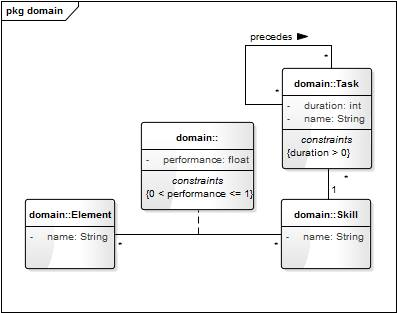
\includegraphics[width=10cm, height = 10cm]{uml.jpg}
  \caption{Diagrama de classes UML}
  \label{fig:uml}
\end{figure}

\subsection{Fases}
\justify\normalsize 
O projeto será dividido em fases de trabalho. A inicial passa pelo desenvolvimento da arquitetura explicitada em cima. Seguidamente, proceder-se-á implementação dos \index{Algortimos Genéticos} algoritmos genéticos. Finalmente, será desenvolvido o arrefecimento simulado. As fases abordadas até ao presente relatório foram as duas primeiras. A arquitetura explicitada pelo diagrama de classes uml já foi implementada e a obtenção de solução por algoritmos genéticos encontra-se numa fase avançada.

\subsection{Algoritmos Genéticos}
\justify\normalsize
Explicar o algoritmo usado:
	- estrutura do cromossoma
	- função de avaliação
	- seleção
	- cruzamento
	- mutações

\subsection{Arrefecimento Simulado}
\justify\normalsize
Explicar o algoritmo usado.

\section{Trabalho Realizado}
\justify\normalsize
Incluir trechos do código já implementado.

\section{Testes}
\justify\normalsize
Explicar os testes planeados.

\section{Conclusões}
\justify\normalsize
Conclusões retiradas.

\printindex

\end{titlepage}
\end{document} to your LaTeX file where you want your
% title page.
%
%%%%%%%%%%%%%%%%%%%%%%%%%%%%%%%%%%%%%%%%%

%----------------------------------------------------------------------------------------
%	PACKAGES AND OTHER DOCUMENT CONFIGURATIONS
%----------------------------------------------------------------------------------------

\documentclass[12pt, showidx]{article}

\usepackage[utf8]{inputenc}
\usepackage[T1]{fontenc}
\usepackage{lmodern}
\usepackage{parselines}
\usepackage[portuguese]{babel}
\usepackage{graphicx}
\usepackage{imakeidx}
\usepackage[document]{ragged2e}

\graphicspath{ {images/} }

\makeindex[title = Palavras Chave]

\begin{document}

\begin{titlepage}

\newcommand{\HRule}{\rule{\linewidth}{1mm}} % Defines a new command for the horizontal lines, change thickness here

\center % Center everything on the page
 
%----------------------------------------------------------------------------------------
%	HEADING SECTIONS
%----------------------------------------------------------------------------------------


\includegraphics{feup.jpg}

\textsc{\large Inteligência Artificial}\\[0.5cm] % Major heading such as course name
\textsc{\large 3º ano do Mestrado Integrado em Engenharia Informática e Computação}\\[0.5cm] % Minor heading such as course title

%----------------------------------------------------------------------------------------
%	TITLE SECTION
%----------------------------------------------------------------------------------------

\HRule \\[0.4cm]
{ \huge \bfseries Otimização da gestão de projetos}\\[0.2cm] % Title of your document
\HRule \\[1cm]
 
%----------------------------------------------------------------------------------------
%	AUTHOR SECTION
%----------------------------------------------------------------------------------------


% If you don't want a supervisor, uncomment the two lines below and remove the section above
\Large \emph{Authors:}\\
Duarte \textsc{Pinto}\\[0cm] - up201304777 
- up201304777@fe.up.pt\\[0cm]
Filipa \textsc{Ramos}\\[0cm] - up201305378
- up201305378@fe.up.pt\\[0cm] 
Gustavo \textsc{Silva}\\[0cm] - up201304143
- up201304143@fe.up.pt\\[1cm] % Your name

%----------------------------------------------------------------------------------------
%	DATE SECTION
%----------------------------------------------------------------------------------------

{\large \today}\\[0cm] % Date, change the \today to a set date if you want to be precise

%----------------------------------------------------------------------------------------
%	TABLE OF CONTENTS & LISTS OF FIGURES AND TABLES
%----------------------------------------------------------------------------------------

\tableofcontents

%----------------------------------------------------------------------------------------
%	INTRODUÇÃO
%----------------------------------------------------------------------------------------

\section{Introdução} 

\justify\normalsize
No âmbito da unidade curricular de Inteligência Artificial pretende-se desenvolver um programa que, com base em algoritmos genéticos e arrefecimento simulado, faça a gestão de um projeto balançando os elementos participantes e as tarefas a realizar do mesmo. O sistema é composto por um conjunto de tarefas que pertencem ao projeto em análise. Cada tarefa tem uma competência indispensável ao seu cumprimento e uma duração. Cada elemento tem um conjunto de competências sendo que o mesmo tem um nível de capacidade para cumprir cada uma. A gestão a ser realizada tem em vista minimizar o tempo ocupado para satisfazer todas as tarefas do projeto usando a melhor combinação de elementos para cada tarefa. Será feita uma análise comparativa entre o desempenho das solução encontradas com algoritmos genéticos e arrefecimento simulado. 

Os objetivos principais do projeto passam pela exploração da implementação prática dos algoritmos genéticos e do algoritmo de arrefecimento simulado. Através dos dados obtidos, visa-se também realizar uma comparação da solução encontrada com ambos os algoritmos. Este processo irá fomentar o conhecimento adquirido, evidenciando as vantagens principais de cada algoritmo e as suas dicotomias principais.  

Espera-se que surjam dificuldades na implementação prática dos algoritmos estudados teoricamente, principalmente na construção dos cromossomas pois existem dúvidas em relação à sua influência na eficiência da solução encontrada. Para além disto, a melhor adaptação da função de avaliação ao problema por forma a obter os melhores resultados revela-se um processo tumultuoso. Os membros decidiram optar por otimizar o tempo utilizado a concluir todas as tarefas do projeto em estudo. Desta forma, a melhor solução será a que implicará um menor tempo de conclusão do projeto em questão.

%----------------------------------------------------------------------------------------

\newpage % Start the article content on the second page, remove this if you have a longer abstract that goes onto the second page

%----------------------------------------------------------------------------------------
%	ESPECIFICAÇÃO
%----------------------------------------------------------------------------------------

\section{Especificação}

\subsection{Problematização}
\justify\normalsize
O sistema tem por objetivo otimizar a atribuição de membros por tarefas num dado projeto. Os dados do mesmo são introduzidos por input através de um ficheiro.

Um projeto em análise caracteriza-se por um conjunto de tarefas (\index{Task} Task) a cumprir, tendo estas um nome (por motivos de identificação) e uma duração. Existe ainda um conjunto de elementos (\index{Element} Element) que podem ser atribuídos a essas mesmas tarefas. Um elemento é identificado por um nome e tem uma lista de competências (\index{Skill} Skill) avaliadas em função da sua capacidade. Por exemplo, o elemento "joão" tem competências na área da informática a um nível 6 e na área da economia com nível 10.

\subsection{Aquitetura}
\justify\normalsize
O projeto foi dividido em três "packages" principais que representam os três níveis mais importantes. Um dos packages diz respeito às classes que guardam informação sobre as tarefas, os elementos e as competências. Os outros dois dizem respeito à implementação do algoritmo genético ou do arrefecimento simulado.

A arquitetura pensada para o projeto passa pela implementação de três classes principais que interagem entre si próprias. A classe "Task" representa uma tarefa e guarda a sua duração. Um elemento é representado pela classe "Element" que mantém a identificação do mesmo. A classe "Skill" corresponde a uma competência. Estas ligam-se entre si por forma a que um elemento tenha vários skills e um skill tenha várias tarefas tal como é visível na figura \ref{fig:uml}.

\begin{figure}[h]
  \centering
    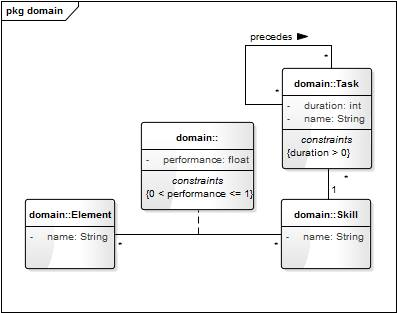
\includegraphics[width=10cm, height = 10cm]{uml.jpg}
  \caption{Diagrama de classes UML}
  \label{fig:uml}
\end{figure}

\subsection{Fases}
\justify\normalsize 
O projeto será dividido em fases de trabalho. A inicial passa pelo desenvolvimento da arquitetura explicitada em cima. Seguidamente, proceder-se-á implementação dos \index{Algortimos Genéticos} algoritmos genéticos. Finalmente, será desenvolvido o arrefecimento simulado. As fases abordadas até ao presente relatório foram as duas primeiras. A arquitetura explicitada pelo diagrama de classes uml já foi implementada e a obtenção de solução por algoritmos genéticos encontra-se numa fase avançada.

\subsection{Algoritmos Genéticos}
\justify\normalsize
Explicar o algoritmo usado:
	- estrutura do cromossoma
	- função de avaliação
	- seleção
	- cruzamento
	- mutações

\subsection{Arrefecimento Simulado}
\justify\normalsize
Explicar o algoritmo usado.

\section{Trabalho Realizado}
\justify\normalsize
Incluir trechos do código já implementado.

\section{Testes}
\justify\normalsize
Explicar os testes planeados.

\section{Conclusões}
\justify\normalsize
Conclusões retiradas.

\printindex

\end{titlepage}
\end{document} to your LaTeX file where you want your
% title page.
%
%%%%%%%%%%%%%%%%%%%%%%%%%%%%%%%%%%%%%%%%%

%----------------------------------------------------------------------------------------
%	PACKAGES AND OTHER DOCUMENT CONFIGURATIONS
%----------------------------------------------------------------------------------------

\documentclass[12pt, showidx]{article}

\usepackage[utf8]{inputenc}
\usepackage[T1]{fontenc}
\usepackage{lmodern}
\usepackage{parselines}
\usepackage[portuguese]{babel}
\usepackage{graphicx}
\usepackage{imakeidx}
\usepackage[document]{ragged2e}

\graphicspath{ {images/} }

\makeindex[title = Palavras Chave]

\begin{document}

\begin{titlepage}

\newcommand{\HRule}{\rule{\linewidth}{1mm}} % Defines a new command for the horizontal lines, change thickness here

\center % Center everything on the page
 
%----------------------------------------------------------------------------------------
%	HEADING SECTIONS
%----------------------------------------------------------------------------------------


\includegraphics{feup.jpg}

\textsc{\large Inteligência Artificial}\\[0.5cm] % Major heading such as course name
\textsc{\large 3º ano do Mestrado Integrado em Engenharia Informática e Computação}\\[0.5cm] % Minor heading such as course title

%----------------------------------------------------------------------------------------
%	TITLE SECTION
%----------------------------------------------------------------------------------------

\HRule \\[0.4cm]
{ \huge \bfseries Otimização da gestão de projetos}\\[0.2cm] % Title of your document
\HRule \\[1cm]
 
%----------------------------------------------------------------------------------------
%	AUTHOR SECTION
%----------------------------------------------------------------------------------------


% If you don't want a supervisor, uncomment the two lines below and remove the section above
\Large \emph{Authors:}\\
Duarte \textsc{Pinto}\\[0cm] - up201304777 
- up201304777@fe.up.pt\\[0cm]
Filipa \textsc{Ramos}\\[0cm] - up201305378
- up201305378@fe.up.pt\\[0cm] 
Gustavo \textsc{Silva}\\[0cm] - up201304143
- up201304143@fe.up.pt\\[1cm] % Your name

%----------------------------------------------------------------------------------------
%	DATE SECTION
%----------------------------------------------------------------------------------------

{\large \today}\\[0cm] % Date, change the \today to a set date if you want to be precise

%----------------------------------------------------------------------------------------
%	TABLE OF CONTENTS & LISTS OF FIGURES AND TABLES
%----------------------------------------------------------------------------------------

\tableofcontents

%----------------------------------------------------------------------------------------
%	INTRODUÇÃO
%----------------------------------------------------------------------------------------

\section{Introdução} 

\justify\normalsize
No âmbito da unidade curricular de Inteligência Artificial pretende-se desenvolver um programa que, com base em algoritmos genéticos e arrefecimento simulado, faça a gestão de um projeto balançando os elementos participantes e as tarefas a realizar do mesmo. O sistema é composto por um conjunto de tarefas que pertencem ao projeto em análise. Cada tarefa tem uma competência indispensável ao seu cumprimento e uma duração. Cada elemento tem um conjunto de competências sendo que o mesmo tem um nível de capacidade para cumprir cada uma. A gestão a ser realizada tem em vista minimizar o tempo ocupado para satisfazer todas as tarefas do projeto usando a melhor combinação de elementos para cada tarefa. Será feita uma análise comparativa entre o desempenho das solução encontradas com algoritmos genéticos e arrefecimento simulado. 

Os objetivos principais do projeto passam pela exploração da implementação prática dos algoritmos genéticos e do algoritmo de arrefecimento simulado. Através dos dados obtidos, visa-se também realizar uma comparação da solução encontrada com ambos os algoritmos. Este processo irá fomentar o conhecimento adquirido, evidenciando as vantagens principais de cada algoritmo e as suas dicotomias principais.  

Espera-se que surjam dificuldades na implementação prática dos algoritmos estudados teoricamente, principalmente na construção dos cromossomas pois existem dúvidas em relação à sua influência na eficiência da solução encontrada. Para além disto, a melhor adaptação da função de avaliação ao problema por forma a obter os melhores resultados revela-se um processo tumultuoso. Os membros decidiram optar por otimizar o tempo utilizado a concluir todas as tarefas do projeto em estudo. Desta forma, a melhor solução será a que implicará um menor tempo de conclusão do projeto em questão.

%----------------------------------------------------------------------------------------

\newpage % Start the article content on the second page, remove this if you have a longer abstract that goes onto the second page

%----------------------------------------------------------------------------------------
%	ESPECIFICAÇÃO
%----------------------------------------------------------------------------------------

\section{Especificação}

\subsection{Problematização}
\justify\normalsize
O sistema tem por objetivo otimizar a atribuição de membros por tarefas num dado projeto. Os dados do mesmo são introduzidos por input através de um ficheiro.

Um projeto em análise caracteriza-se por um conjunto de tarefas (\index{Task} Task) a cumprir, tendo estas um nome (por motivos de identificação) e uma duração. Existe ainda um conjunto de elementos (\index{Element} Element) que podem ser atribuídos a essas mesmas tarefas. Um elemento é identificado por um nome e tem uma lista de competências (\index{Skill} Skill) avaliadas em função da sua capacidade. Por exemplo, o elemento "joão" tem competências na área da informática a um nível 6 e na área da economia com nível 10.

\subsection{Aquitetura}
\justify\normalsize
O projeto foi dividido em três "packages" principais que representam os três níveis mais importantes. Um dos packages diz respeito às classes que guardam informação sobre as tarefas, os elementos e as competências. Os outros dois dizem respeito à implementação do algoritmo genético ou do arrefecimento simulado.

A arquitetura pensada para o projeto passa pela implementação de três classes principais que interagem entre si próprias. A classe "Task" representa uma tarefa e guarda a sua duração. Um elemento é representado pela classe "Element" que mantém a identificação do mesmo. A classe "Skill" corresponde a uma competência. Estas ligam-se entre si por forma a que um elemento tenha vários skills e um skill tenha várias tarefas tal como é visível na figura \ref{fig:uml}.

\begin{figure}[h]
  \centering
    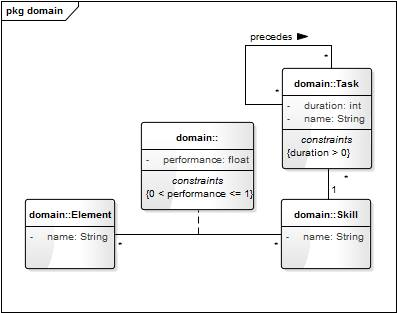
\includegraphics[width=10cm, height = 10cm]{uml.jpg}
  \caption{Diagrama de classes UML}
  \label{fig:uml}
\end{figure}

\subsection{Fases}
\justify\normalsize 
O projeto será dividido em fases de trabalho. A inicial passa pelo desenvolvimento da arquitetura explicitada em cima. Seguidamente, proceder-se-á implementação dos \index{Algortimos Genéticos} algoritmos genéticos. Finalmente, será desenvolvido o arrefecimento simulado. As fases abordadas até ao presente relatório foram as duas primeiras. A arquitetura explicitada pelo diagrama de classes uml já foi implementada e a obtenção de solução por algoritmos genéticos encontra-se numa fase avançada.

\subsection{Algoritmos Genéticos}
\justify\normalsize
Explicar o algoritmo usado:
	- estrutura do cromossoma
	- função de avaliação
	- seleção
	- cruzamento
	- mutações

\subsection{Arrefecimento Simulado}
\justify\normalsize
Explicar o algoritmo usado.

\section{Trabalho Realizado}
\justify\normalsize
Incluir trechos do código já implementado.

\section{Testes}
\justify\normalsize
Explicar os testes planeados.

\section{Conclusões}
\justify\normalsize
Conclusões retiradas.

\printindex

\end{titlepage}
\end{document} to your LaTeX file where you want your
% title page.
%
%%%%%%%%%%%%%%%%%%%%%%%%%%%%%%%%%%%%%%%%%

%----------------------------------------------------------------------------------------
%	PACKAGES AND OTHER DOCUMENT CONFIGURATIONS
%----------------------------------------------------------------------------------------

\documentclass[12pt, showidx]{article}

\usepackage[utf8]{inputenc}
\usepackage[T1]{fontenc}
\usepackage{lmodern}
\usepackage{parselines}
\usepackage[portuguese]{babel}
\usepackage{graphicx}
\usepackage{imakeidx}
\usepackage[document]{ragged2e}

\graphicspath{ {images/} }

\makeindex[title = Palavras Chave]

\begin{document}

\begin{titlepage}

\newcommand{\HRule}{\rule{\linewidth}{1mm}} % Defines a new command for the horizontal lines, change thickness here

\center % Center everything on the page
 
%----------------------------------------------------------------------------------------
%	HEADING SECTIONS
%----------------------------------------------------------------------------------------


\includegraphics{feup.jpg}

\textsc{\large Inteligência Artificial}\\[0.5cm] % Major heading such as course name
\textsc{\large 3º ano do Mestrado Integrado em Engenharia Informática e Computação}\\[0.5cm] % Minor heading such as course title

%----------------------------------------------------------------------------------------
%	TITLE SECTION
%----------------------------------------------------------------------------------------

\HRule \\[0.4cm]
{ \huge \bfseries Otimização da gestão de projetos}\\[0.2cm] % Title of your document
\HRule \\[1cm]
 
%----------------------------------------------------------------------------------------
%	AUTHOR SECTION
%----------------------------------------------------------------------------------------


% If you don't want a supervisor, uncomment the two lines below and remove the section above
\Large \emph{Authors:}\\
Duarte \textsc{Pinto}\\[0cm] - up201304777 
- up201304777@fe.up.pt\\[0cm]
Filipa \textsc{Ramos}\\[0cm] - up201305378
- up201305378@fe.up.pt\\[0cm] 
Gustavo \textsc{Silva}\\[0cm] - up201304143
- up201304143@fe.up.pt\\[1cm] % Your name

%----------------------------------------------------------------------------------------
%	DATE SECTION
%----------------------------------------------------------------------------------------

{\large \today}\\[0cm] % Date, change the \today to a set date if you want to be precise

%----------------------------------------------------------------------------------------
%	TABLE OF CONTENTS & LISTS OF FIGURES AND TABLES
%----------------------------------------------------------------------------------------

\tableofcontents

%----------------------------------------------------------------------------------------
%	INTRODUÇÃO
%----------------------------------------------------------------------------------------

\section{Introdução} 

\justify\normalsize
No âmbito da unidade curricular de Inteligência Artificial pretende-se desenvolver um programa que, com base em algoritmos genéticos e arrefecimento simulado, faça a gestão de um projeto balançando os elementos participantes e as tarefas a realizar do mesmo. O sistema é composto por um conjunto de tarefas que pertencem ao projeto em análise. Cada tarefa tem uma competência indispensável ao seu cumprimento e uma duração. Cada elemento tem um conjunto de competências sendo que o mesmo tem um nível de capacidade para cumprir cada uma. A gestão a ser realizada tem em vista minimizar o tempo ocupado para satisfazer todas as tarefas do projeto usando a melhor combinação de elementos para cada tarefa. Será feita uma análise comparativa entre o desempenho das solução encontradas com algoritmos genéticos e arrefecimento simulado. 

Os objetivos principais do projeto passam pela exploração da implementação prática dos algoritmos genéticos e do algoritmo de arrefecimento simulado. Através dos dados obtidos, visa-se também realizar uma comparação da solução encontrada com ambos os algoritmos. Este processo irá fomentar o conhecimento adquirido, evidenciando as vantagens principais de cada algoritmo e as suas dicotomias principais.  

Espera-se que surjam dificuldades na implementação prática dos algoritmos estudados teoricamente, principalmente na construção dos cromossomas pois existem dúvidas em relação à sua influência na eficiência da solução encontrada. Para além disto, a melhor adaptação da função de avaliação ao problema por forma a obter os melhores resultados revela-se um processo tumultuoso. Os membros decidiram optar por otimizar o tempo utilizado a concluir todas as tarefas do projeto em estudo. Desta forma, a melhor solução será a que implicará um menor tempo de conclusão do projeto em questão.

%----------------------------------------------------------------------------------------

\newpage % Start the article content on the second page, remove this if you have a longer abstract that goes onto the second page

%----------------------------------------------------------------------------------------
%	ESPECIFICAÇÃO
%----------------------------------------------------------------------------------------

\section{Especificação}

\subsection{Problematização}
\justify\normalsize
O sistema tem por objetivo otimizar a atribuição de membros por tarefas num dado projeto. Os dados do mesmo são introduzidos por input através de um ficheiro.

Um projeto em análise caracteriza-se por um conjunto de tarefas (\index{Task} Task) a cumprir, tendo estas um nome (por motivos de identificação) e uma duração. Existe ainda um conjunto de elementos (\index{Element} Element) que podem ser atribuídos a essas mesmas tarefas. Um elemento é identificado por um nome e tem uma lista de competências (\index{Skill} Skill) avaliadas em função da sua capacidade. Por exemplo, o elemento "joão" tem competências na área da informática a um nível 6 e na área da economia com nível 10.

\subsection{Aquitetura}
\justify\normalsize
O projeto foi dividido em três "packages" principais que representam os três níveis mais importantes. Um dos packages diz respeito às classes que guardam informação sobre as tarefas, os elementos e as competências. Os outros dois dizem respeito à implementação do algoritmo genético ou do arrefecimento simulado.

A arquitetura pensada para o projeto passa pela implementação de três classes principais que interagem entre si próprias. A classe "Task" representa uma tarefa e guarda a sua duração. Um elemento é representado pela classe "Element" que mantém a identificação do mesmo. A classe "Skill" corresponde a uma competência. Estas ligam-se entre si por forma a que um elemento tenha vários skills e um skill tenha várias tarefas tal como é visível na figura \ref{fig:uml}.

\begin{figure}[h]
  \centering
    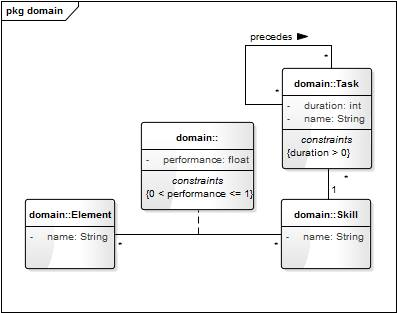
\includegraphics[width=10cm, height = 10cm]{uml.jpg}
  \caption{Diagrama de classes UML}
  \label{fig:uml}
\end{figure}

\subsection{Fases}
\justify\normalsize 
O projeto será dividido em fases de trabalho. A inicial passa pelo desenvolvimento da arquitetura explicitada em cima. Seguidamente, proceder-se-á implementação dos \index{Algortimos Genéticos} algoritmos genéticos. Finalmente, será desenvolvido o arrefecimento simulado. As fases abordadas até ao presente relatório foram as duas primeiras. A arquitetura explicitada pelo diagrama de classes uml já foi implementada e a obtenção de solução por algoritmos genéticos encontra-se numa fase avançada.

\subsection{Algoritmos Genéticos}
\justify\normalsize
Explicar o algoritmo usado:
	- estrutura do cromossoma
	- função de avaliação
	- seleção
	- cruzamento
	- mutações

\subsection{Arrefecimento Simulado}
\justify\normalsize
Explicar o algoritmo usado.

\section{Trabalho Realizado}
\justify\normalsize
Incluir trechos do código já implementado.

\section{Testes}
\justify\normalsize
Explicar os testes planeados.

\section{Conclusões}
\justify\normalsize
Conclusões retiradas.

\printindex

\end{titlepage}
\end{document}